\chapter{Trace analysis}

\section{Parsing}
Although the format presented in chapter \ref{v8-instrumentation} is really simple, parsing it can prove to be challenging.
The sole reason is the size of the files. It is really common for websites to produce files of size in the range of a few Gigabytes.
Some can even output as much as 48 GB in about 2 minutes!

The analyzing program was written in Haskell \cite{haskell:main-page}.
Haskell is a purely functional, lazy, statically typed language.
It has been chosen because it is relatively easy to write parsers in a language like this.
Further, static typing with pattern matching proves convenient when manipulating well-structured data like log entries.
Last but not least, automatically derived instances
\footnote{Without going into details, classes in Haskell are a bit like interfaces in 
object-oriented languages, e.g. class \emph{Ord} defines objects that can be compared}
help avoid writing tedious code and focus on implementing non-trivial parts.

All that being said, Haskell is a bit like C++ -- inexperienced user can easily make mistakes
that render the code slow and memory-greedy.

The logging format was described in section \ref{v8-bytecode-injection}.
Each entry consist of event type, and several locations. Each location comprises
function name, source file and position in the file.

At first, internal format for the event was exactly the same. One object consisted of
two strings and two numbers (it could be one number, but this way line and column info
logging can be turned on any time).

The first mistake, specific to Haskell, was to use \emph{String} type to represent function and file
names. The use of default \emph{String} to represent textual data makes the code inefficient 
because it is a linked lists of \emph{Char}s, i.e. to store one character 9 bytes of memory are used.
It is so wrong and inefficient to use this type that it is not worth trying to profile such implementation.

That error was fixed by changing the representation to \emph{ByteString} type from \emph{bytesting} 
package \cite{haskell:bytestring}. \emph{ByteString}s are represented internally as real byte arrays,
not linked lists. 
This change was accompanied by rewrite of the parsing code to \emph{attoparsec} \cite{haskell:attoparsec},
which can operate of \emph{ByteString}s as an input.

The code was now much less memory-consuming and faster, but it still seemed to consume too much memory.
Profiling proved that suspicions were warranted. The profiling diagram is shown on figure \ref{fig:bytestring-lazy}. 
All profiling diagrams in this section were collected by running the analyzing program on the same set of 6 input files.
First three occupy 48MB each, the last three 4MB each.
All files combined occupy around 150MB, while peak memory usage of the program is above 900MB.

\begin{figure}[hbt!]
 \centering
 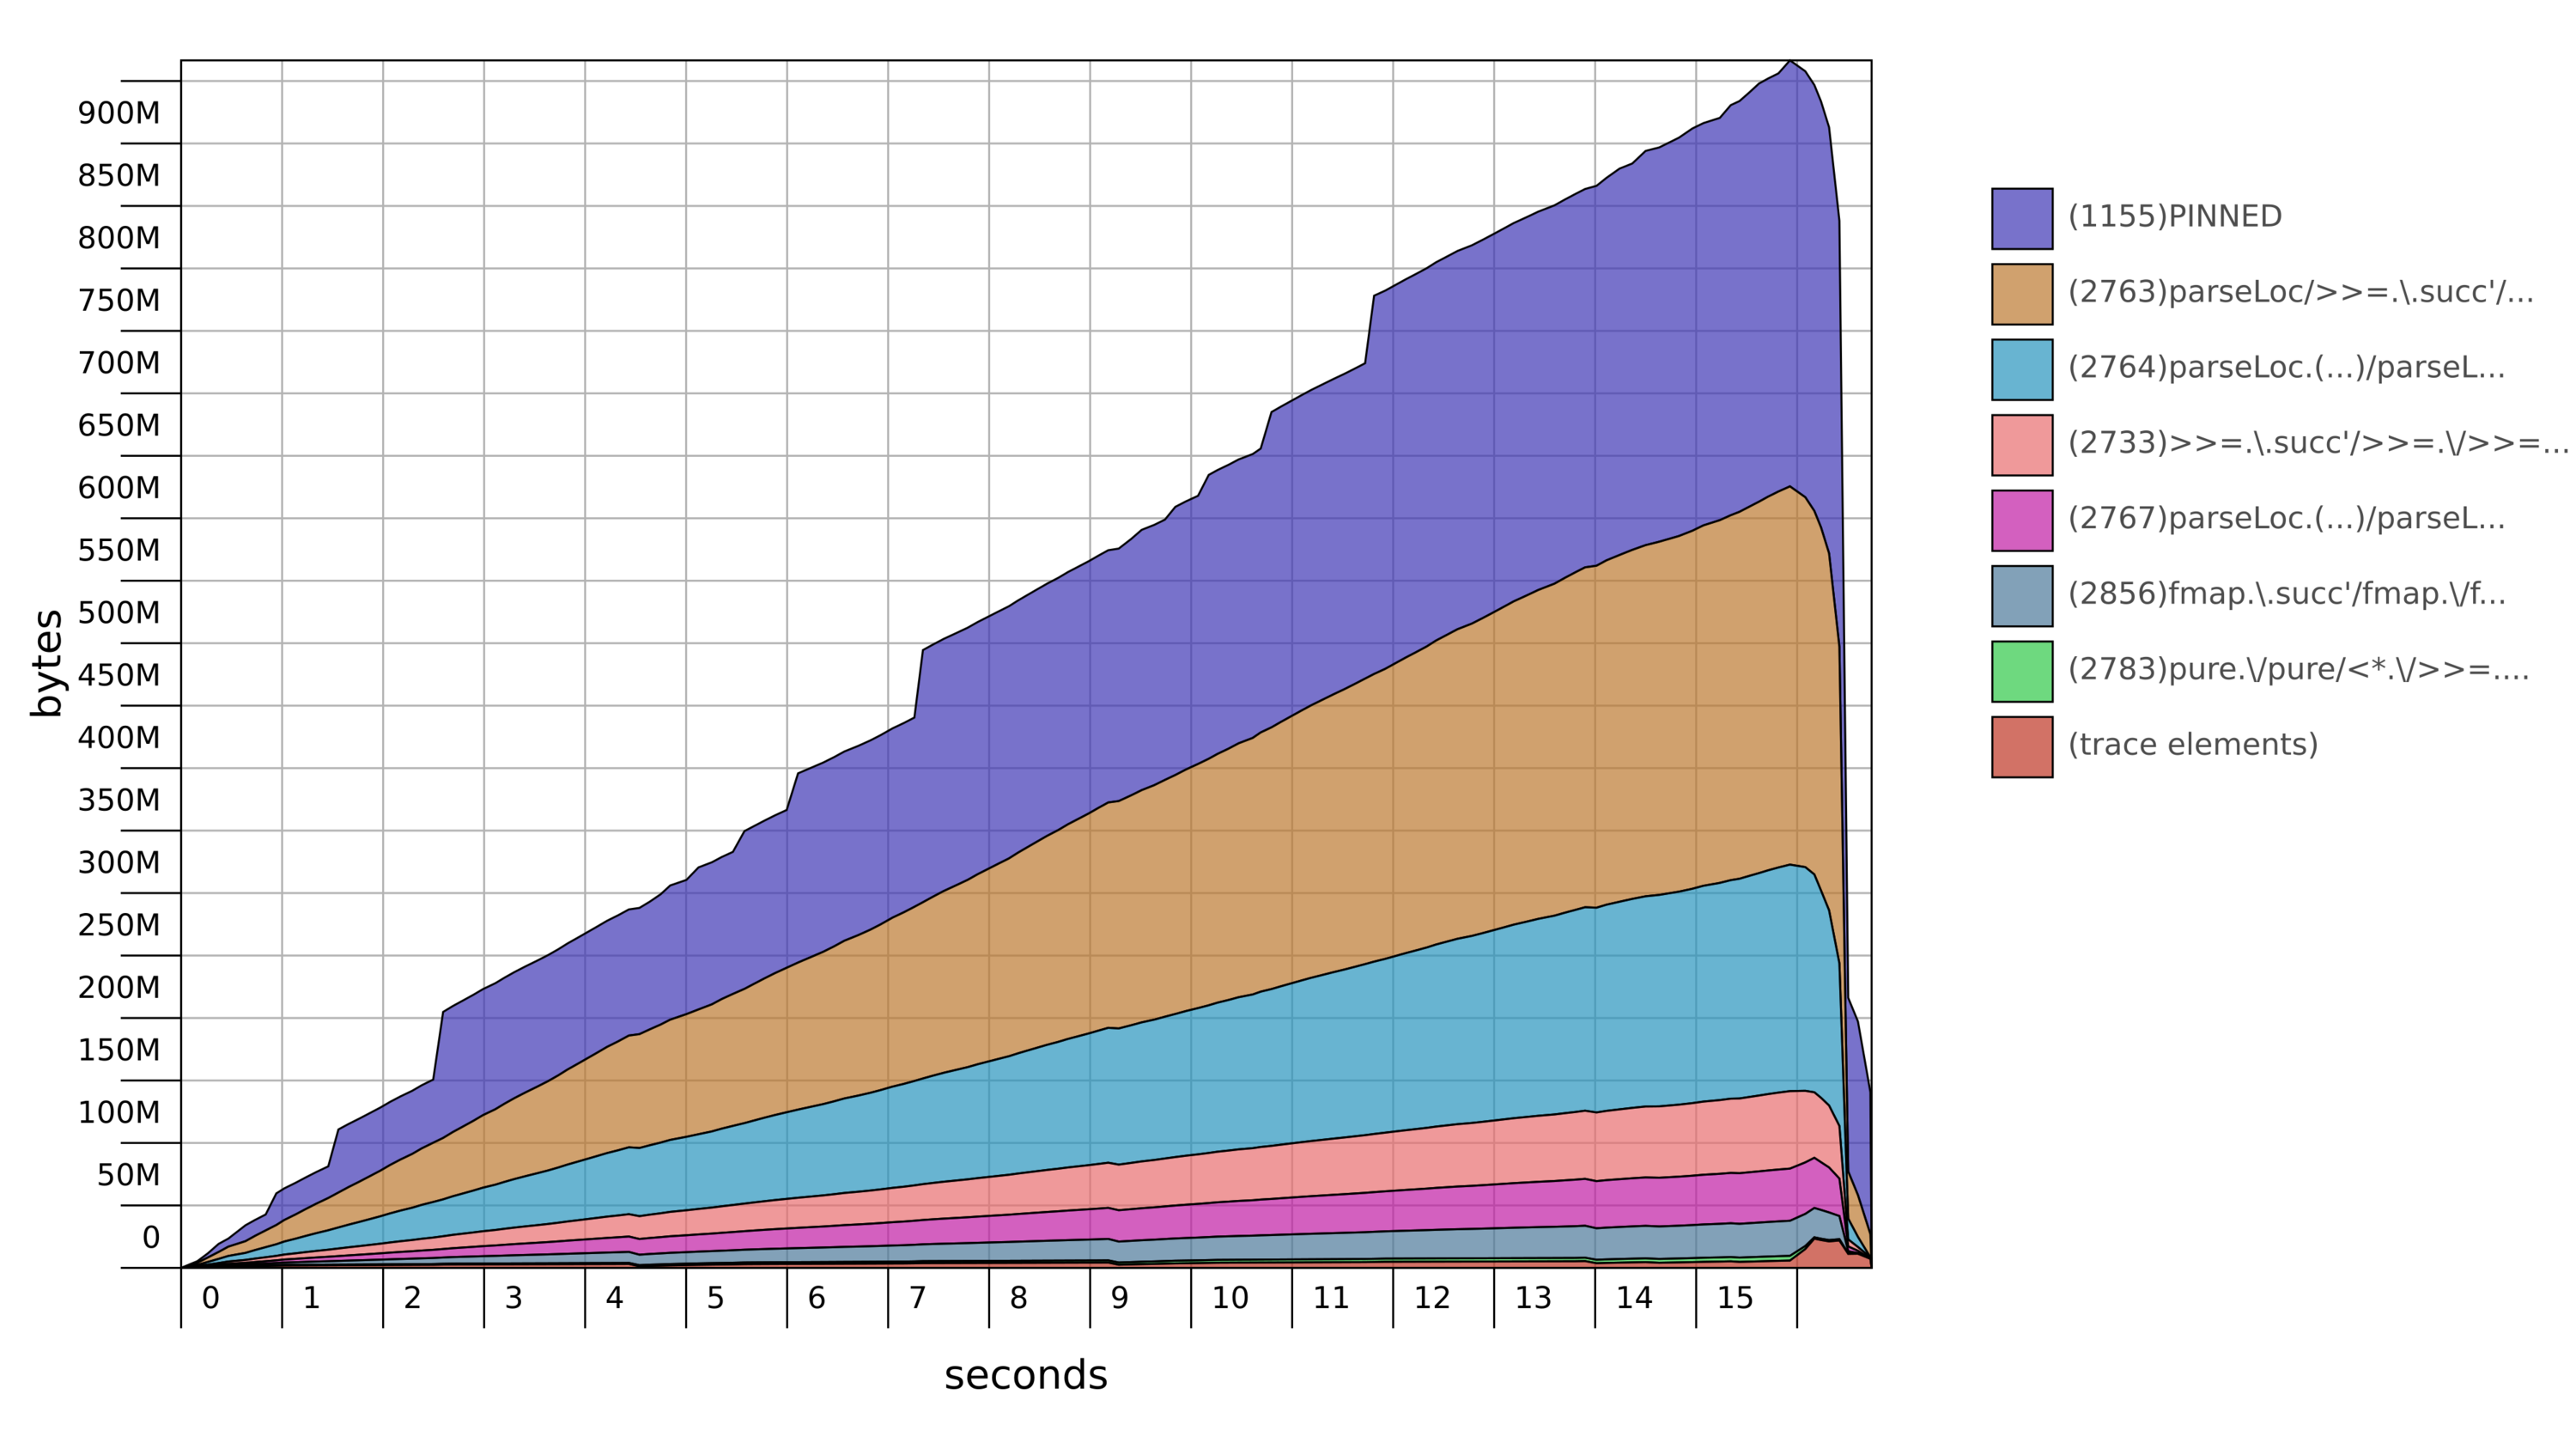
\includegraphics[width=\textwidth]{png/bytestring-lazy}
 \caption{Memory usage of the first implementation using ByteStrings as internal strings representation}
 \label{fig:bytestring-lazy}
\end{figure}

Looking at the diagram, pinned memory seemed to be never freed during the execution. 
Also, traces seemed to reside in memory for too long and occupy too much space. 

The first problem was a reflection of how Haskell keeps \emph{ByteString}s.
They are stored in pinned memory, which is kept on a heap but 
not managed by garbage collector \cite{haskell:shortbytestring-and-text} and cannot be moved around.
As a result, it leads to fragmentation of the heap and cannot be effectively managed.
The fix turned out to be simple. There is a more suitable storage format -- \emph{ShortByteString} 
(also part of the \emph{bytestring} package). It is managed
by GC and stored just like usual heap object, which can be moved around and easily garbage collected.
\footnote{So why even use \emph{ByteString}? Because it is stored in pinned memory, it can be passed to foreign functions.
Also, it is more efficient when the strings are really long and have long livespan}

The second problem was harder to track down. This time the cause was the laziness.
Laziness can improve the perfomance when some objects are never used and the language never needs to fully compute them. 
However, when we know that all objects will eventually be used, it is more efficient
to calculate them as soon as possible. The enforcement of eager evaluation seems to be an obscure
feature, but when we know what is going on, it is fine.
The improvement was visible (figure \ref{fig:shortbytestring-strict}) but it was not the end, 
as peak usage of almost 240MB is still greater than 150MB.

\begin{figure}[hbt!]
 \centering
 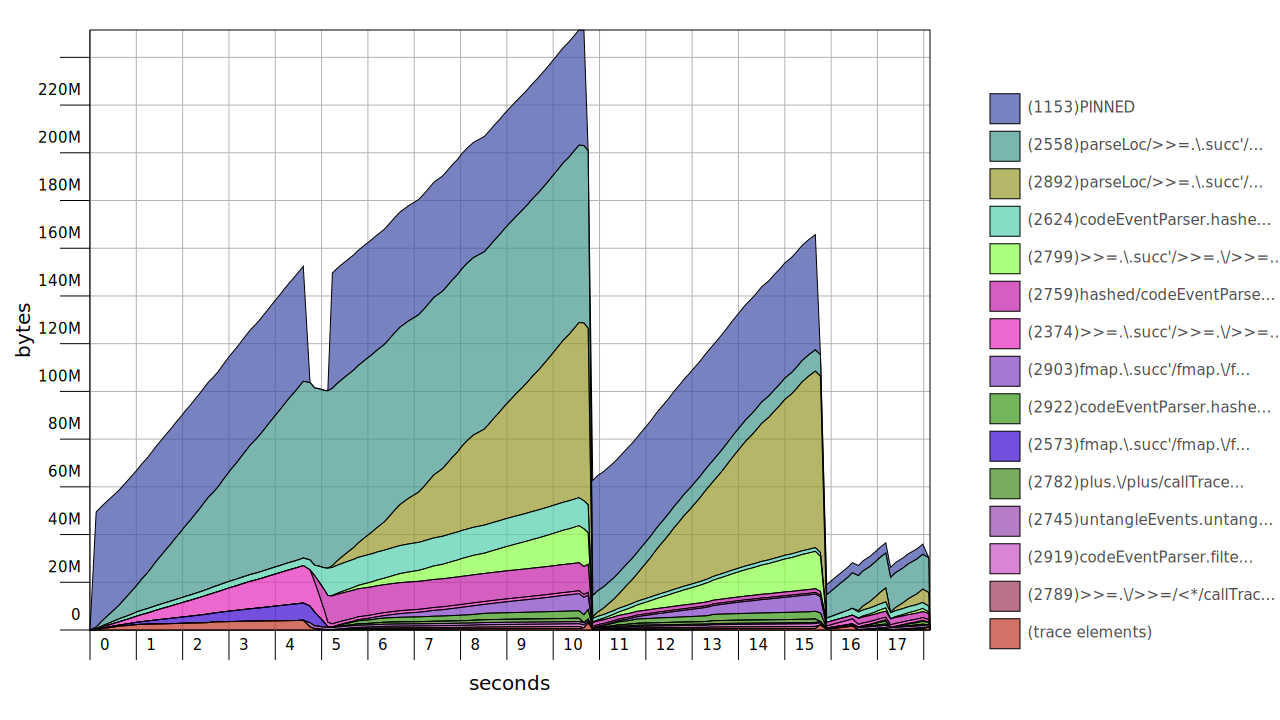
\includegraphics[width=\textwidth]{png/shortbytestring-strict}
 \caption{Memory usage after switching to ShortByteString and forcing eager evaluation}
 \label{fig:shortbytestring-strict}
\end{figure}

It seems suspicious that the entire file has to be kept in memory to be parsed 
(pinned memory on figure \ref{fig:shortbytestring-strict} represents input files read into memory). 
After all, if it was written in C++, probably one line at a time would be read and processed. 
So why this parser consumes so much memory?

This is what \emph{attoparsec} states about incremental input:

\begin{displayquote}
Note: incremental input does not imply that attoparsec will release portions of its internal state for 
garbage collection as it proceeds. Its internal representation is equivalent to a single ByteString: 
if you feed incremental input to a parser, it will require memory proportional to the amount of input you supply. 
(This is necessary to support arbitrary backtracking.)
\end{displayquote}

So, our parser keeps the whole file contents in memory to be able to backtrack. But it is not necessary with
such a simple format. Fortunately, it is possible to improve this behaviour.
Currently, the parser tries to parse the entire file into a list of events. To be sure that it can backtrack,
it keeps the whole input in memory. Instead, we can ask the parser to parse only one event. 
It will do it and return the part of the input that was not parsed yet. We can repeat that in a loop
and parser will never keep more memory that just a few kilobytes. 
Figure \ref{fig:single-event} shows the improvement.

\begin{figure}[hbt!]
 \centering
 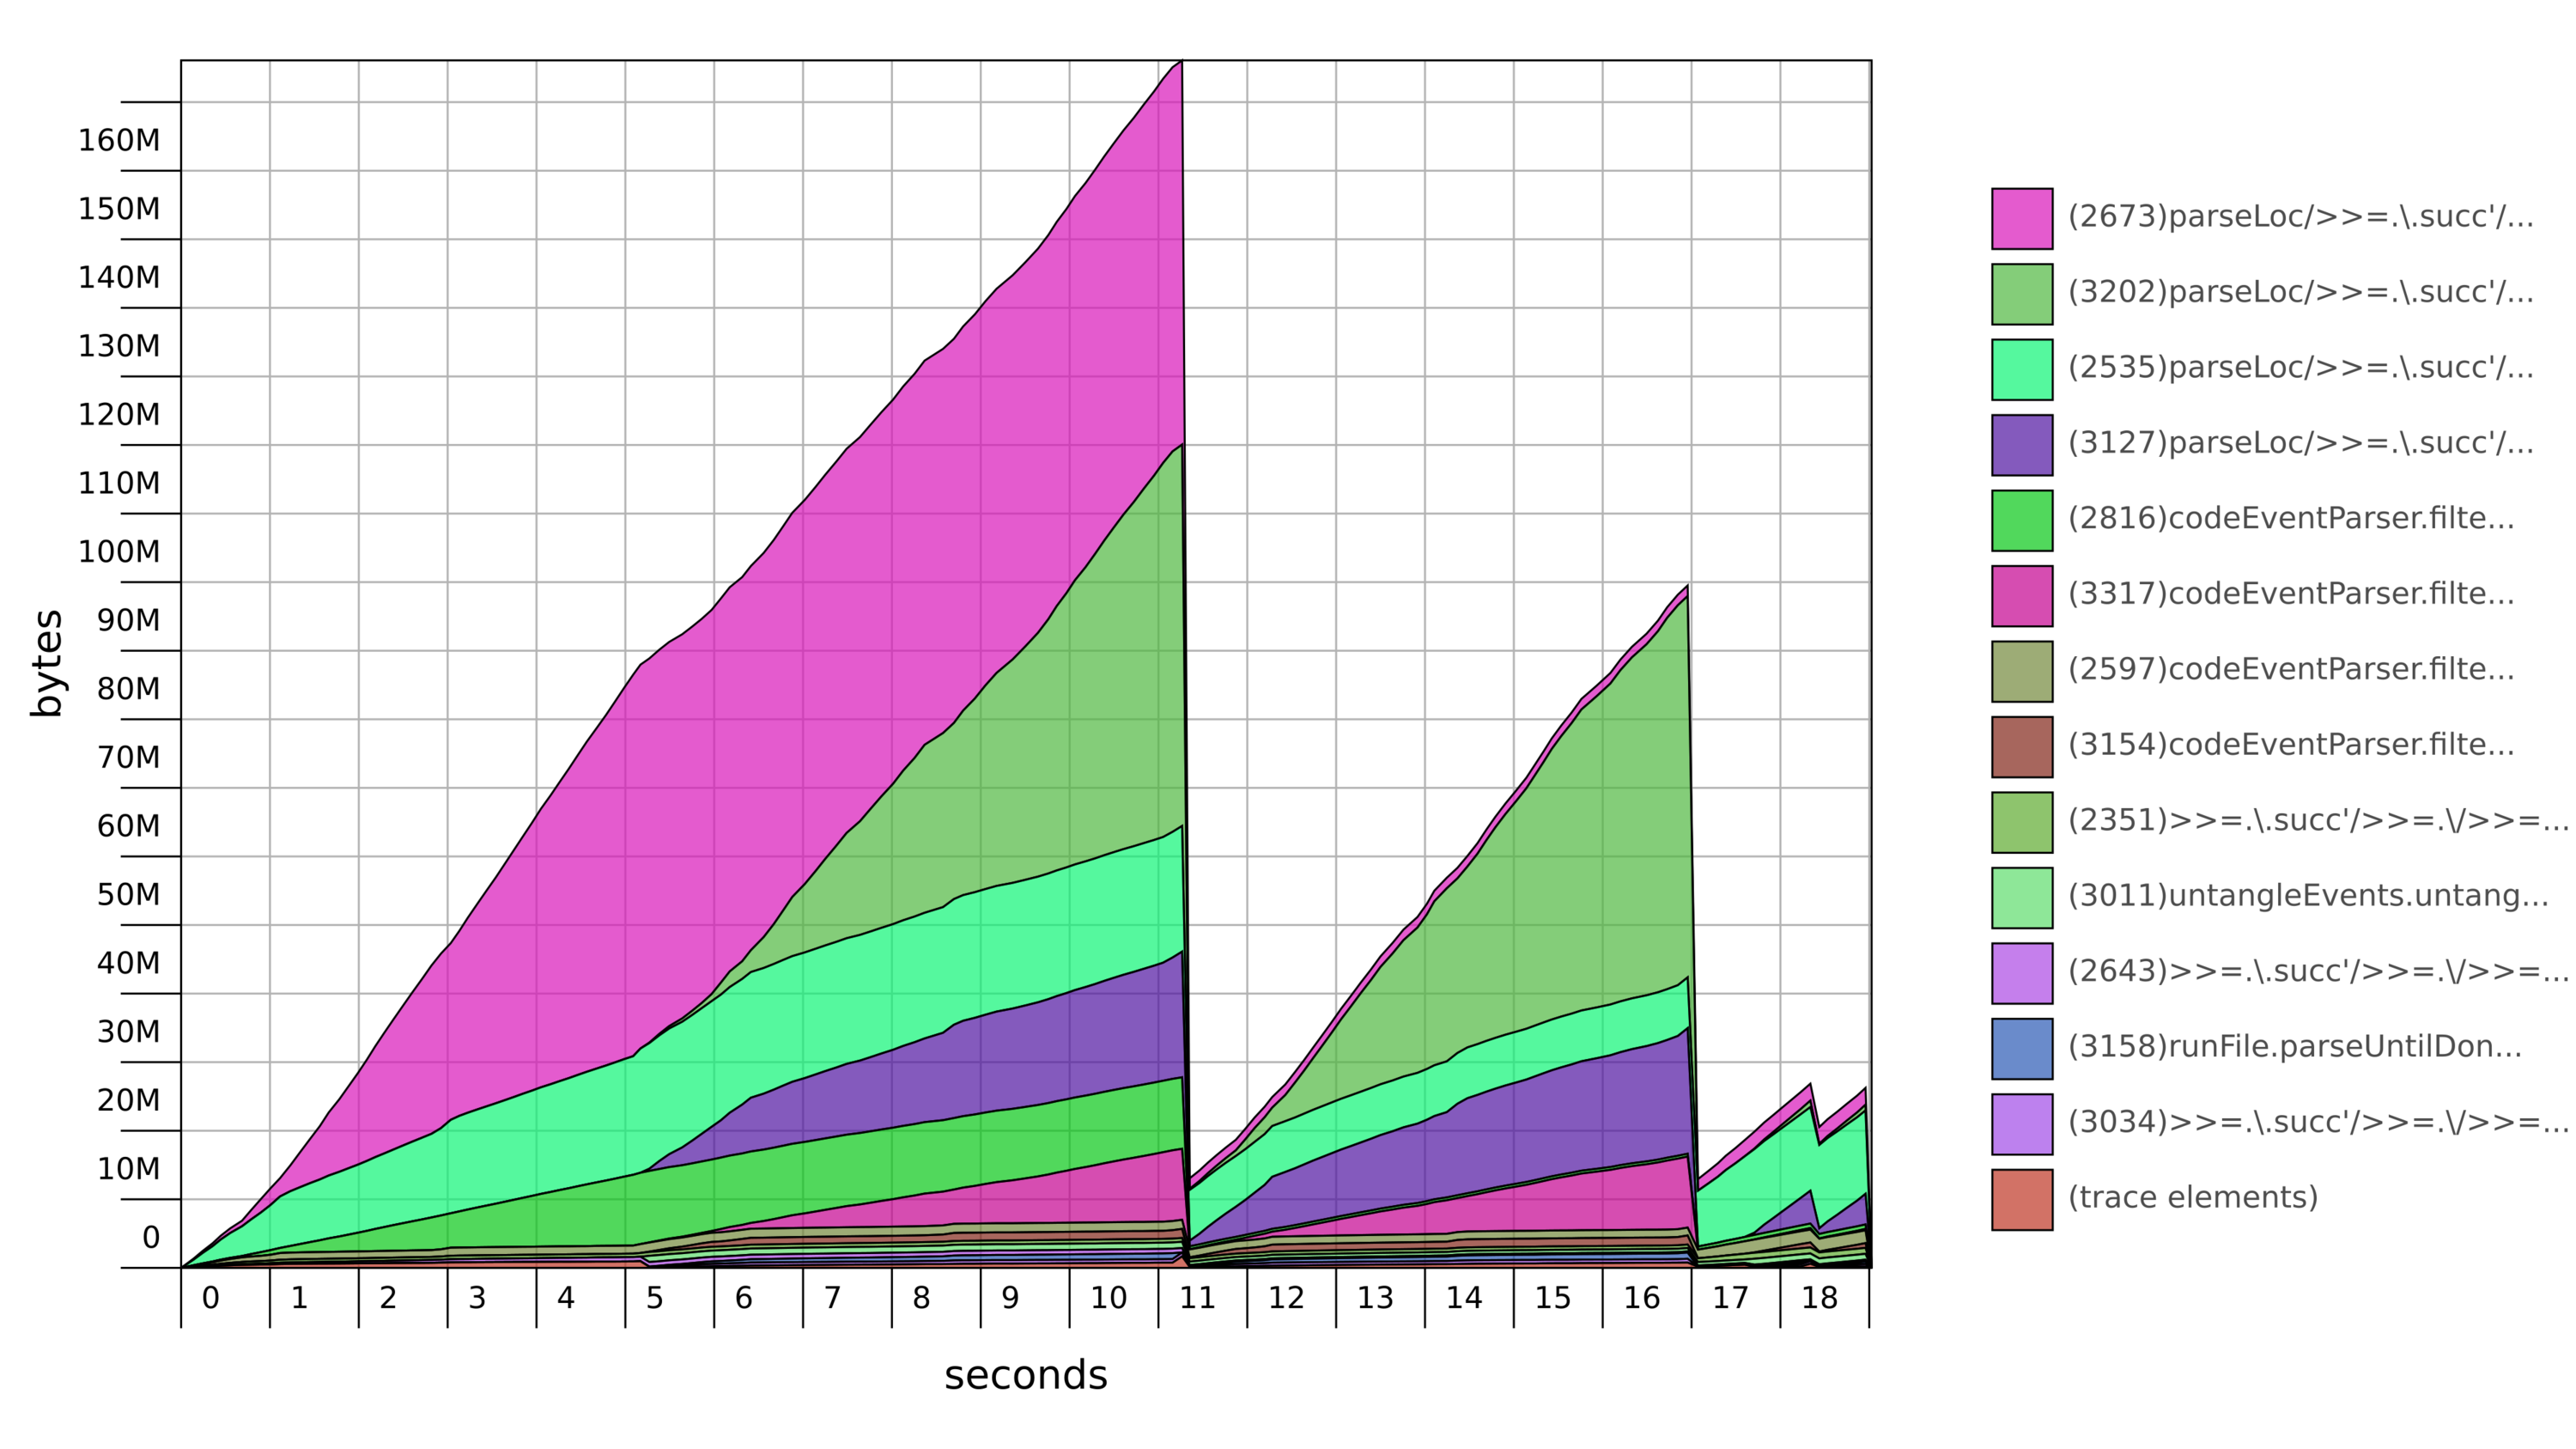
\includegraphics[width=\textwidth]{png/single-event}
 \caption{Memory usage after preventing parser from keeping the entire input file in the memory}
 \label{fig:single-event}
\end{figure}

Last, but not least, the internal representation of the event can be greatly improved.
Locations consist of file names and function names. But both sets are limited!
Usualy there are only a few sources containing just a few hundreds of unique functions. 
We can create a map of all source and function names and just keep appropriate ids in location objects.
Just 4 numbers instead of 2 strings and 2 numbers!

This representation also has another major benefit -- comparisons of such objects are much fasters.

The final memory consumption is presented in figure \ref{fig:strings-map}

\begin{figure}[hbt!]
 \centering
 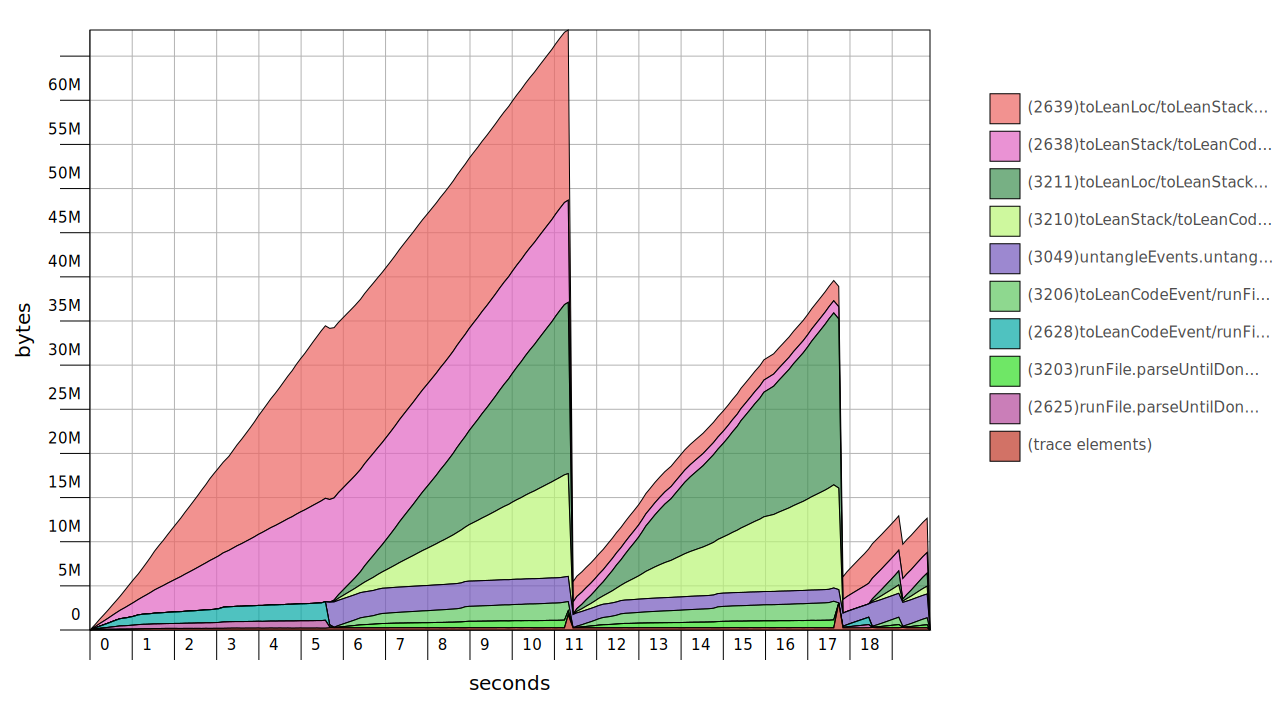
\includegraphics[width=\textwidth]{png/strings-map}
 \caption{Final memory usage}
 \label{fig:strings-map}
\end{figure}


\section{Trace untangling}
Due to the nature of JavaScript execution model (see section \ref{js-exec-model}), execution events
corresponding to different JavaScript events or functions can be intertwined.

For this reason, all events forming a trace have to be untangled into subtraces, each corresponding
to one script or callback. 

Let us recall that all events are logged by our instumented Chromium with their call stacks.
Now, we have three cases:
\begin{itemize}
  \item The event is a function enter with an empty call stack -- it starts a new subtrace
  \item The event is a function exit removing the last item from the stack -- it ends a subtrace
  \item Any other event -- it is a continuation of a subtrace, whose last event has the same call stack
\end{itemize}

Naturally, some care has to be taken to ensure that the right stack is compared. Some events change the
call stack, e.g. function enter and exit, some do not, e.g. "if statement -- then".
Here, the stack \emph{after} the event occured is saved and it is appopriately modified 
(one location can be added, removed or nothing is changed) when comparing
with past events stacks.

Listing \ref{alg:untangling} presents the pseudocode of the algorithm.

\lstinputlisting[language=Pseudocode, caption=Pseudocode of the trace untangling algorithm, label=alg:untangling, mathescape=true]{algorithms/untangling.alg}

The above code is rather uncomplicated, but it is slow when implemented naively.
The most wasteful part is finding the trace with the right stack in \emph{findMatchingSubtrace}.
To make it faster, two things were done:
\begin{itemize}
  \item Location objects are just 4 numbers instead of 2 strings and 2 numbers. This makes stack comparisons
           one or two orders of magnitude faster
  \item Open traces are kept in a map indexed by stack of the last event. 
  			The lookup becomes logarithmic instead of linear. This optimization is especially important when there are lots
  			of intertwined subtraces. It also must be noted that this optimization alone would not help much if the comparisons 
  			between stacks were slow
\end{itemize} 

One last caveat -- it is possible to enter a function in JavaScript and never return.
When an exception is thrown and there is no catch block in a function, the error will
be propagated higher and control can possibly leave multiple functions without any of them returning any value.
Those throw events will not be logged, therefore this situation has to be taken care of
in the analyzing program. The solution is the following: when there is no open subtrace with a matching stack,
the program will check if some stack will match with any number of elements removed from the top.
If yes, then we assume that it is due to the try-catch block.


\section{Trace alignment}
\label{trace-alignment}

Trace alignment is a technique of identyfing execution differences of two runs of the same program.
To be able to align two traces, events in both have to be assigned execution indices.
In our the execution index is the event type, its location and stack at the time of its occurence.
In this thesis execution event is often used interchangeably execution event as everything that is
logged when an event occurs is the index.

The algorithm used in this implementation is based on an article by Johnson et al. \cite{ieee:alignment-and-slicing}
The result of trace alignment is an execution trace diff. It is a list of events of three kinds:
\begin{itemize}
  \item Common -- an event that occured in both traces
  \item Left -- an event that occured only in the left trace
  \item Right -- an event that occured only in the right trace
\end{itemize}

Each diff event includes the assiciated execution event.
Listing \ref{alg:alignment} present the pseudocode of the algorithm.

\lstinputlisting[language=Pseudocode, caption=Pseudocode of the trace alignment algorithm, 
                       label=alg:alignment, mathescape=true]{algorithms/alignment.alg}
                       
The algorithm output includes a score, which is a number of common events.
This concept was not present in the original article and its purpose 
will be explained in section \ref{trace-matching}.

The algorithm is rather simple. We assume that matching traces have to start with the same
event. If they do not (lines 5-6), we just terminate and return score of -1, 
which signifies that traces do not match.

Apart from the case when one of the traces ends, there are only two cases:
\begin{itemize}
  \item Both unprocessed traces start with the same event (that includes stacks equality), line 20 -- in that case
  			we add an event of type Common and remove one event from both lists
  \item The top events do not match (lines 25 and 28) -- in that case the event with larger stack is removed first.
           The reasoning is the following. The bottom of the larger stack is the same as the shorter stack.
           If we first process the shorter stack and if it shrinks, we lose some common events later.
           It we process the larger stack first, the shorter one is "frozen". The larger stack may grow, but it doesn't matter
           since it is already divergent. When it shrinks to the size of the shorter stack, it will be a reconvergence point.
\end{itemize}


\section{Trace matching using Stable Marriage Problem}
\label{trace-matching}

We already know how to align two traces (section \ref{trace-alignment}), but we have not
answered a different question -- which pair of subtraces should we align?

This thesis presents a novel approach, which uses Stable Marriage Problem to answer this question.
First, we should define what SMP is and later explain how it is adapted to our needs.

The original statement of the problem is the following \cite{wiki:smp}: 
given equallly sized sets of men and women and their matrimonial preferences,
find a stable matching, i.e. matching in which there exists no pair of man and woman 
in which they both would have better partner than the currently assigned one.

The problem can be solved using Gale-Shapley algorithm. Listing \ref{alg:gale-shapley} presents its pseudocode.

\lstinputlisting[language=Pseudocode, caption=Pseudocode of the Gale-Shapley (deferred acceptance) algorithm, 
                       label=alg:gale-shapley, mathescape=true]{algorithms/gale-shapley.alg}

This is how SMP is used to solve subtrace matching problem:
\begin{itemize}
  \item In the first phase all pair of subtraces are aligned and similarity score (number of common events) 
  		    is calculated -- the score is the marital preference
  \item In the second phase, adapted Gale-Shapley algorithm is run and only matched subtraces
           are used. Their diff is simply retrived from a special map as it was calculated already in the first phase.
\end{itemize}

All men have a list of women sorted by their preferences (from highest to lowest).
At the beginning everyone is free. Then, in each round each free man m proposes to first woman w he has not yet proposed to.
Woman can reply "maybe" if she is free or is engaged to m' and prefers m over m'. Otherwise she rejects.
So women only "trade up" and men propose whenever they are free to the best possible partner.
In the end everybody is engaged and the marriages are stable.

Time complexity of this algorithm is $O(n^2)$, where $n$ is the number of men or women.
There is at most $n$ rounds (some man proposes to every woman) and in each round
there are at most $n$ proposals made.

In the original problem statement the number of woman is equal to the number of men
and everybody gets engaged in the end.
In our case the number of men and women does not have to the same. We assume that
the more numerous group has the role of women. 
We allow some pairs of men and women to not match to each other (preference score equal to -1),
therefore in the end some people may not be engaged.

Let us see what happens with these two changes and the same procedure as in the original version:
\begin{itemize}
  \item The men should still propose in the order from highest preference to the lowest. 
  			All man will still get the best possible match this way, 
  			because all women that rejected must have had some better options.
  \item The women should accept anybody when they do not have any tentative match and
           only trade up later. If there is a man that a woman prefers over a current match and he did not
           propose, he must have had someone who he preferred more and who accepted.
\end{itemize}

Consequently, the algoritm is almost the same. The only exception is that men do not propose to women with score -1.
Also, the result is different -- in the end there usually will be many people without a pair. 
However, those who have a pair will form a stable marriage.

Such usage of Stable Matching Algorithm allows us to form the best pairs of subtraces to align.
There is no point in aligning the traces that do not have the same initial event (the aligning algoritm has to
start from an anchor point), so we skip those pairs with assigning score -1. Further, the best pairs are
selected by the number of common event. If two traces A and B are exactly the same, the only possibility that they will
not be matched is when there is one longer trace C that contain entire A and B. But, it there is also a longer trace D
that contains entire A and B, it is very likely that the extra part will be matched with extra part of C and,
is consequence, C and D will be matched. If there is no such trace D and C is matched is either A or B, it is still
fine, as we have more calls to some function in one group and we cannot be sure which subtraces truly
correspond to each other.


\section{Artificial examples}

This section presents the algorithm work on some simple, hand-crafted examples run in standalone V8.

First example is based on our already-familiar example of \emph{factorial} (listing \ref{js-factorial}).

First, we will call the function with $n=3$, then with $n=4$ and compare the traces.
This demonstrates how "if-then-else" divergences are detected.
Listing \ref{diff:factorial} shows the output of the program.

We see that after 3 \emph{factorial} calls the traces diverge and one of them takes the "else"
path and makes one more recursive call (lines 19-30). The other taken the "then" path (lines 31-33).
After than one extra recursive call both traces immediately reconverge (line 34).

\lstinputlisting[language=TraceDiff, caption={Trace diff of \emph{factorial} run with n=3 and n=4},  label=diff:factorial]{out/factorial.diff}

The next example demonstrates that sometimes it is possible to find a divergence even when
built-in functions are involved. Listing \ref{js:map} is a short example involving \emph{Array.prototype.map}.
In the first run it was called with an array of length 3, in the second the array had one less item.
Listing \ref{diff:map} shows the diff. We can see that in one run \emph{multiplyByTwo} is entered 2 times and in the
other 3 times. Naturally, if the arrays were of the same length, but with different content, this difference would not
be caught this way.

\lstinputlisting[language=JavaScript, caption=Simple JavaScript example of \emph{Array.prototype.map} usage, label=js:map]{js/map.js}

\lstinputlisting[language=TraceDiff, caption={Trace diff of \emph{Array.prototype.map} run with array of length 3 and 2},  
						label=diff:map]{out/map.diff}
						
The last example example demonstrates generator-related events in action.
Listing \ref{js:generators} shows an example of factorial rewritten to use generators. It was run two times, with $n=2$ and $n=3$.
Listing \ref{diff:generators} shows the resulting diff. We can see that when the generator is created, "Function Enter" event
is emitted, followed by "Generator Suspend" (lines 7-12). Events "Generator Enter" and "Generator Yield" are used 
only when \emph{Generator.prototype.next} is called. Last, but not least, "Generator Yield" is always followed by "Generator Suspend".

\lstinputlisting[language=JavaScript, caption=Example of JavaScript code using generators, label=js:generators]{js/generators.js}

\lstinputlisting[language=TraceDiff, caption={Trace diff of generator-using \emph{factorial} run with n=2 and n=3},  
						label=diff:generators]{out/generators.diff}

\section{Noise filtering}

One of the biggest challenges in the entire method is filtering the noise.
The noise on the website comes in many different flavours:
\begin{itemize}
  \item Some content can based on Random Number Generators.
  \item Content may be dynamic and different with each refresh of the page, e.g. Facebook feed.
  \item Code that is not related to the website, e.g. trackers, analytics
\end{itemize}

The difficult part is to filter out as much data as possible without removing valuable information.

In the original article authors collected redundant traces, diffed together all positive traces (and then also negative traces)
and generated a blacklist of execution differences that are guaranteed to be noise.

Here the approach is different. The positive traces are all put together and the common subtraces are extracted.
The same thing is done with the negative traces. 
At the end the whole SMP and alignment analysis (see sections \ref{trace-alignment} and \ref{trace-matching}) 
is run only on those common subtraces.

The effectiveness and limitations of this approach will be discussed in the chapter \ref{evaluation}.



